\documentclass[main.tex]{subfiles}

%\externalcitedocument{bibfile}

\begin{document}

\subsection{Systematic Downsizing}

\subsection{DOM Efficiency}

To evaluate the effects of varrying the DOM efficiency on reconstructed event rates, a Monte Carlo sample was generated following the Snowstorm method for low-level systematic uncertainties.

For each batch of ten simulated MC events the DOM effeiciency is sampled from its prior. 
The wavelength acceptance of the DOMS in CLSim is then adjusted according to the new DOM model, and the photon propagation is carried out. 
The remainder of the MC simulation chain is then performed.
The final-level MC is then weighted, one at a time, to the conventional, prompt, and astrophysical neutrino fluxes. 

In order to calculate the effects of perturbing the DOM effeiciency on the reconstrucion-level quantities, we bin events in terms of $\log_{E_{\nu}^{reco}}$, $\cos\theta_{\nu}^{reco}$, and the events' sampled DOM efficiencies. 
We then account for the sampling bias in each DOM efficiency bin by integrating the prior PDF over the each DOM efficiency bin and scaling up the weights of events in those bins by one over the cummulative probability of sampling that given bin. 
The sum of the weights in each bin therefore would be a function only of (1) the central expectation in that bin and (2) the bias generated by using a perturbed DOM efficiency. 
For each ($\log E_{\nu}^{reco}$, $\cos\theta_{\nu}^{reco}$) slice, each DOM efficiency bin is then rescaled around the central bin's value; this yields a quantity in each bin that represents the proportional effect of perturbing the DOM efficiency. 

Then, a spline fit is carried out over the full 3D binned space using Photospline~\cite{WHITEHORN20132214}. 
Events can then be reweighted to a new DOM efficiency by evaluating the spline $\mathcal{S}$ at the event's reconstructed energy and zenith, and the new DOM effieciency $\mathcal{D}_{OM}$; this is shown in Equation~EQ.
\begin{equation}\label{eq:domeff}
    w' = w + w\times \mathcal{S}(\log E_{\nu}^{reco}, \cos\theta_{\nu}^{reco}, \mathcal{D}_{OM})
\end{equation}

A slice of the full 3D fit for the conventional neutrino fluxes is shown in Figure~\ref{fig:domeff_fit}.
\begin{figure}
    \centering
    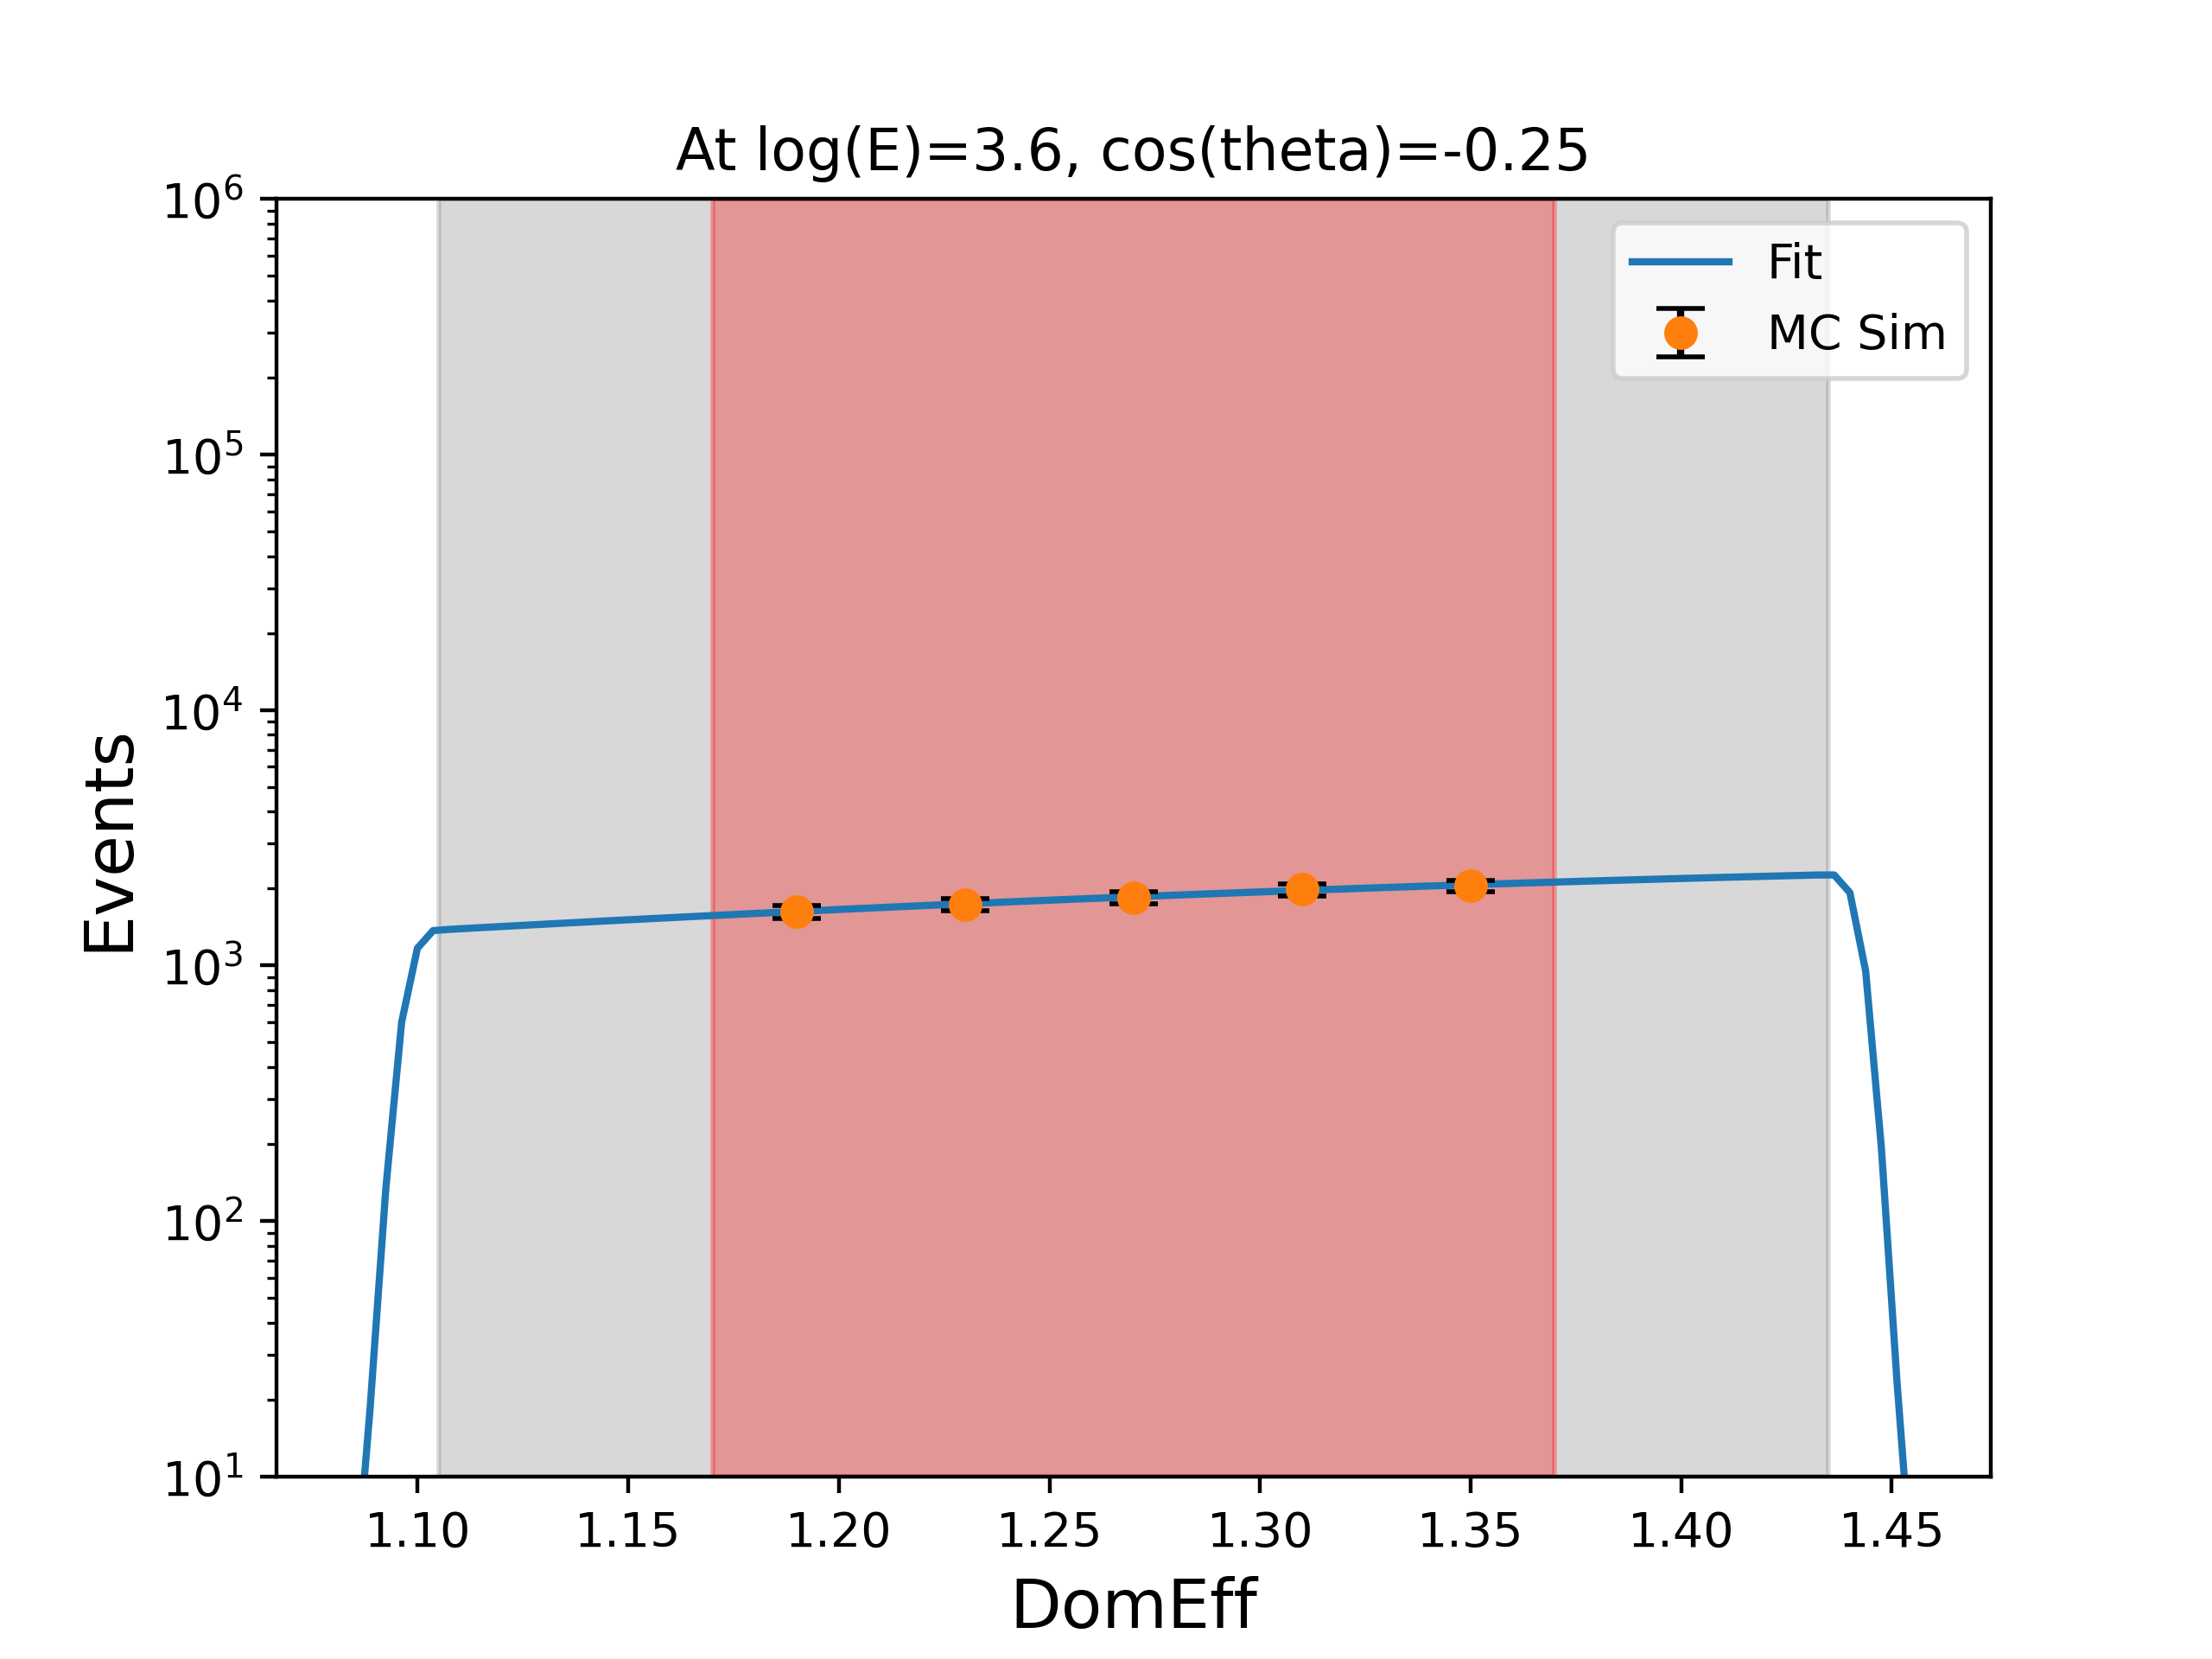
\includegraphics[width=0.8\linewidth]{figures/atmConv_logE_3.6_cosz_-0.25.png}
    \caption{The predicted number of events in reconstructed space for a bin centered at $\log E_{\nu}^{reco}=3.6$ and $\cos\theta_{\nu}^{reco}=0.25$ as a function of the DOM effeciency. The MC data are represented by orange dots, and the spline fit is the trend in blue. The gray shaded region represent the extents of the spline, and the red bands represents prior-allowed region.}\label{fig:domeff_fit}
\end{figure}


\subsection{Bulk Ice}

\subsection{Hole Ice}

The hole ice represents a bubbly, refrozen region of ice around the DOMs. 
The bubbles, which formed during the refreezing, greatly decrease the scattering length of light. 
This has the effect of changing the light-acceptance of the DOMs as a function of photon incident angle. 
A plethora of different angular acceptance curves existed from various different calibration studies done to understand this region of the ice; and work was carried out to approximate these different curves and the space they spanned. 
Spline-fits were carried out using seven support points and by forcing the acceptance to zero at the DOM backside (opposite the PMT). 
This resulted in six free, correlated, parameters needed to describe the acceptance curve. 
A principal component analysis was carried out, and it was found that all acceptance curves span a phase space of lower dimensionality. 
Only two components were needed to describe the space of angular acceptance curves, and those were named $p_{0}$ and $p_{1}$.
In doing so, a small amount of error is introduced, though the overall uncertainty on the hole ice that remains is far greater than the introduced error. 

By construction, these parameters' priors are independent.
The effects of varrying these two parameters is then demonstrated in Figures~\ref{fig:holeiceparmas}.

\begin{figure}
    \centering
    \begin{subfigure}{.45\textwidth}
        \centering
        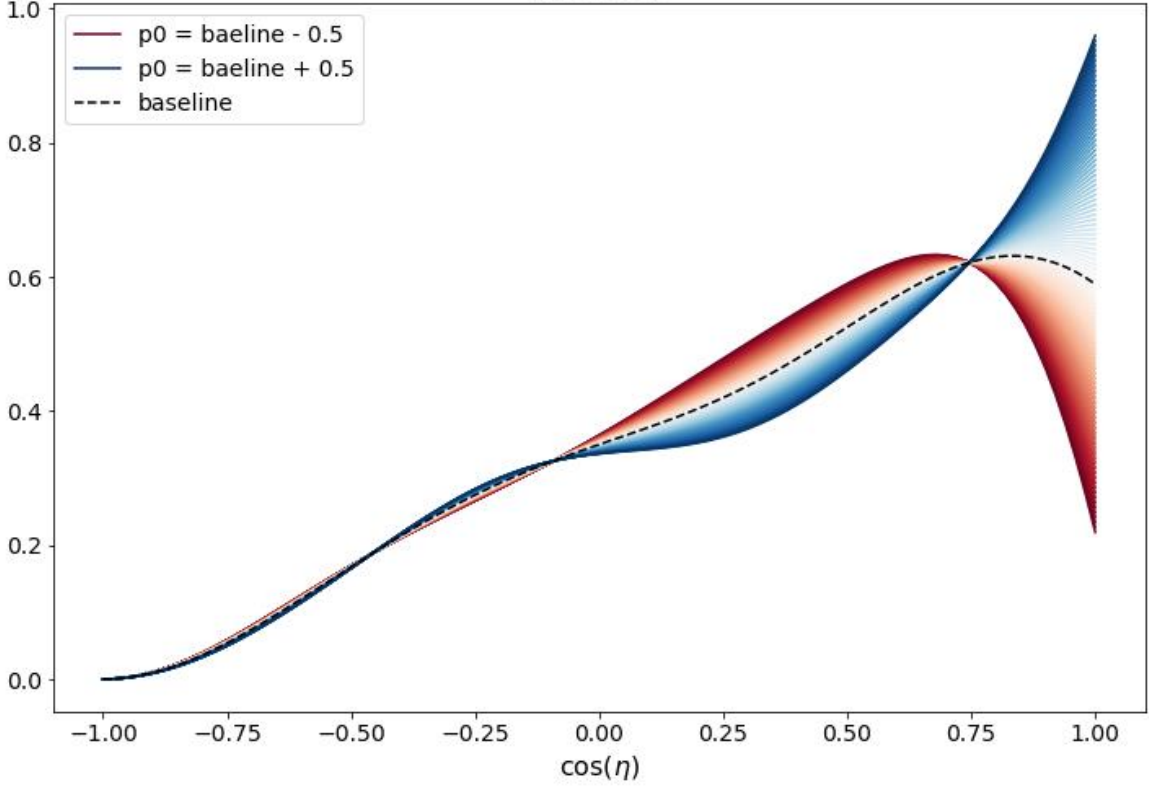
\includegraphics[width=0.95\linewidth]{./figures/holeice_p0.png}
        \caption{A sweep of the unified hole ice model $p_0$ parameter.}
    \end{subfigure}%
    \begin{subfigure}{.45\textwidth}
        \centering
        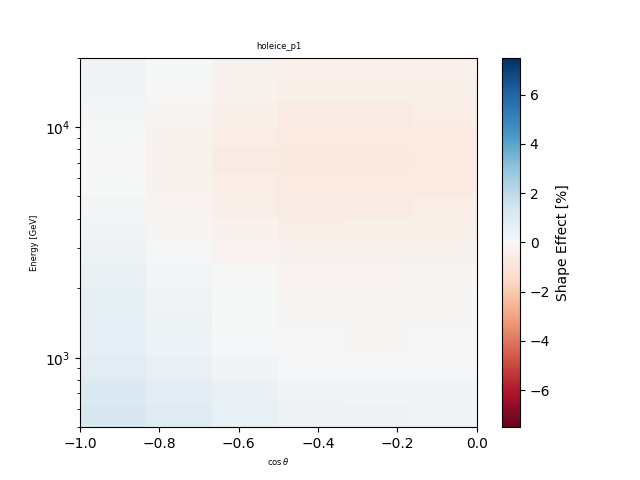
\includegraphics[width=0.95\linewidth]{./figures/holeice_p1.png}
        \caption{A sweep of the unified hole ice model $p_0$ parameter.}
    \end{subfigure}
    \caption{Effects of varrying unified hole ice model parameters. $\eta$ represents angle of photon incidence on the DOM; -1 is the DOM backside, and +1 is the DOM PMT face.}\label{fig:holeiceparmas}
\end{figure}

For each batch of ten simulated MC events these parameters $p_{0}$ and $p_{1}$ are randomly sampled from their priors. 
The angular acceptance of the DOMs in CLSim is then manually adjusted according to the new hole ice model, and the photon propagation is then carried out. 
The remainder of the MC simulation chain is then performed.

The final-level MC is then weighted, one at a time, to the conventional, prompt, and astrophysical neutrino fluxes. 
The snowstorm technique is applied to this MC sample, and the 1D gradients in reconstructed space are shown in Figure FIG. 

\subsection{Atmospheric Neutrino Flux}

Daemonflux and such

\subsection{Atmospheric Density}

\subsection{Keon-nuclei Total Cross Section}

\subsection{Astrophysical Neutrino Flux}

\subsection{Neutrino-Nucleon Interaction}

\end{document}